
\documentclass[a4paper,11pt]{article}
\usepackage[a4paper, margin=8em]{geometry}

% usa i pacchetti per la scrittura in italiano
\usepackage[french,italian]{babel}
\usepackage[T1]{fontenc}
\usepackage[utf8]{inputenc}
\frenchspacing 

% usa i pacchetti per la formattazione matematica
\usepackage{amsmath, amssymb, amsthm, amsfonts}

% usa altri pacchetti
\usepackage{gensymb}
\usepackage{hyperref}
\usepackage{standalone}

\usepackage{colortbl}

\usepackage{xstring}
\usepackage{karnaugh-map}

% imposta il titolo
\title{Electronics for Embedded Systems notes}
\author{Luca Seggiani}
\date{2026}

% spaziatura liste
\usepackage{enumitem}
\setlist[itemize]{noitemsep, topsep=4pt, partopsep=0pt, parsep=2pt, leftmargin=*}
\setlist[enumerate]{noitemsep, topsep=4pt, partopsep=0pt, parsep=2pt, leftmargin=*}

% imposta lo stile
% usa helvetica
\usepackage[scaled]{helvet}
% usa palatino
\usepackage{palatino}
% usa un font monospazio guardabile
\usepackage{lmodern}

\renewcommand{\rmdefault}{ppl}
\renewcommand{\sfdefault}{phv}
\renewcommand{\ttdefault}{lmtt}

% circuiti
\usepackage{circuitikz}
\usetikzlibrary{babel}

% testo cerchiato
\newcommand*\circled[1]{\tikz[baseline=(char.base)]{
            \node[shape=circle,draw,inner sep=2pt] (char) {#1};}}

% disponi il titolo
\makeatletter
\renewcommand{\maketitle} {
	\begin{center} 
		\begin{minipage}[t]{.8\textwidth}
			\textsf{\huge\bfseries \@title} 
		\end{minipage}%
		\begin{minipage}[t]{.2\textwidth}
			\raggedleft \vspace{-1.65em}
			\textsf{\small \@author} \vfill
			\textsf{\small \@date}
		\end{minipage}
		\par
	\end{center}

	\thispagestyle{empty}
	\pagestyle{fancy}
}
\makeatother

% disponi teoremi
\usepackage{tcolorbox}
\newtcolorbox[auto counter, number within=section]{theorem}[2][]{%
	colback=blue!10, 
	colframe=blue!40!black, 
	sharp corners=northwest,
	fonttitle=\sffamily\bfseries, 
	title=Theorem~\thetcbcounter: #2, 
	#1
}

% disponi definizioni
\newtcolorbox[auto counter, number within=section]{definition}[2][]{%
	colback=red!10,
	colframe=red!40!black,
	sharp corners=northwest,
	fonttitle=\sffamily\bfseries,
	title=Definition~\thetcbcounter: #2,
	#1
}

% disponi codice
\usepackage{listings}
\usepackage[table]{xcolor}

\definecolor{codegreen}{rgb}{0,0.6,0}
\definecolor{codegray}{rgb}{0.5,0.5,0.5}
\definecolor{codepurple}{rgb}{0.58,0,0.82}
\definecolor{backcolour}{rgb}{0.95,0.95,0.92}

\lstdefinestyle{codestyle}{
		backgroundcolor=\color{black!5}, 
		commentstyle=\color{codegreen},
		keywordstyle=\bfseries\color{magenta},
		numberstyle=\sffamily\tiny\color{black!60},
		stringstyle=\color{green!50!black},
		basicstyle=\ttfamily\footnotesize,
		breakatwhitespace=false,         
		breaklines=true,                 
		captionpos=b,                    
		keepspaces=true,                 
		numbers=left,                    
		numbersep=5pt,                  
		showspaces=false,                
		showstringspaces=false,
		showtabs=false,                  
		tabsize=2
}

\lstdefinestyle{shellstyle}{
		backgroundcolor=\color{black!5}, 
		basicstyle=\ttfamily\footnotesize\color{black}, 
		commentstyle=\color{black}, 
		keywordstyle=\color{black},
		numberstyle=\color{black!5},
		stringstyle=\color{black}, 
		showspaces=false,
		showstringspaces=false, 
		showtabs=false, 
		tabsize=2, 
		numbers=none, 
		breaklines=true
}

\lstdefinelanguage{x86}{ 
  keywords={AAA, AAD, AAM, AAS, ADC, ADCB, ADCW, ADCL, ADD, ADDB, ADDW, ADDL, AND, ANDB, ANDW, ANDL,
        ARPL, BOUND, BSF, BSFL, BSFW, BSR, BSRL, BSRW, BSWAP, BT, BTC, BTCB, BTCW, BTCL, BTR, 
        BTRB, BTRW, BTRL, BTS, BTSB, BTSW, BTSL, CALL, CBW, CDQ, CLC, CLD, CLI, CLTS, CMC, CMP,
        CMPB, CMPW, CMPL, CMPS, CMPSB, CMPSD, CMPSW, CMPXCHG, CMPXCHGB, CMPXCHGW, CMPXCHGL,
        CMPXCHG8B, CPUID, CWDE, DAA, DAS, DEC, DECB, DECW, DECL, DIV, DIVB, DIVW, DIVL, ENTER,
        HLT, IDIV, IDIVB, IDIVW, IDIVL, IMUL, IMULB, IMULW, IMULL, IN, INB, INW, INL, INC, INCB,
        INCW, INCL, INS, INSB, INSD, INSW, INT, INT3, INTO, INVD, INVLPG, IRET, IRETD, JA, JAE,
        JB, JBE, JC, JCXZ, JE, JECXZ, JG, JGE, JL, JLE, JMP, JNA, JNAE, JNB, JNBE, JNC, JNE, JNG,
        JNGE, JNL, JNLE, JNO, JNP, JNS, JNZ, JO, JP, JPE, JPO, JS, JZ, LAHF, LAR, LCALL, LDS,
        LEA, LEAVE, LES, LFS, LGDT, LGS, LIDT, LMSW, LOCK, LODSB, LODSD, LODSW, LOOP, LOOPE,
        LOOPNE, LSL, LSS, LTR, MOV, MOVB, MOVW, MOVL, MOVSB, MOVSD, MOVSW, MOVSX, MOVSXB,
        MOVSXW, MOVSXL, MOVZX, MOVZXB, MOVZXW, MOVZXL, MUL, MULB, MULW, MULL, NEG, NEGB, NEGW,
        NEGL, NOP, NOT, NOTB, NOTW, NOTL, OR, ORB, ORW, ORL, OUT, OUTB, OUTW, OUTL, OUTSB, OUTSD,
        OUTSW, POP, POPL, POPW, POPB, POPA, POPAD, POPF, POPFD, PUSH, PUSHL, PUSHW, PUSHB, PUSHA, 
        RCLL, RCR, RCRB, RCRW, RCRL, RDMSR, RDPMC, RDTSC, REP, REPE, REPNE, RET, ROL, ROLB, ROLW,
        ROLL, ROR, RORB, RORW, RORL, SAHF, SAL, SALB, SALW, SALL, SAR, SARB, SARW, SARL, SBB,
        SBBB, SBBW, SBBL, SCASB, SCASD, SCASW, SETA, SETAE, SETB, SETBE, SETC, SETE, SETG, SETGE,
        SETL, SETLE, SETNA, SETNAE, SETNB, SETNBE, SETNC, SETNE, SETNG, SETNGE, SETNL, SETNLE,
        SETNO, SETNP, SETNS, SETNZ, SETO, SETP, SETPE, SETPO, SETS, SETZ, SGDT, SHL, SHLB, SHLW,
        SHLL, SHLD, SHR, SHRB, SHRW, SHRL, SHRD, SIDT, SLDT, SMSW, STC, STD, STI, STOSB, STOSD,
        STOSW, STR, SUB, SUBB, SUBW, SUBL, TEST, TESTB, TESTW, TESTL, VERR, VERW, WAIT, WBINVD,
        XADD, XADDB, XADDW, XADDL, XCHG, XCHGB, XCHGW, XCHGL, XLAT, XLATB, XOR, XORB, XORW, XORL},
  keywordstyle=\color{blue}\bfseries,
  ndkeywordstyle=\color{darkgray}\bfseries,
  identifierstyle=\color{black},
  sensitive=false,
  comment=[l]{\#},
  morecomment=[s]{/*}{*/},
  commentstyle=\color{purple}\ttfamily,
  stringstyle=\color{red}\ttfamily,
  morestring=[b]',
  morestring=[b]"
}

\lstdefinelanguage{riscv}{
  keywords={
    LUI, AUIPC,
    JAL, JALR,
    BEQ, BNE, BLT, BGE, BLTU, BGEU,
    LB, LH, LW, LBU, LHU, LD,
    SB, SH, SW, SD,
    ADDI, SLTI, SLTIU, XORI, ORI, ANDI,
    SLLI, SRLI, SRAI,
    ADD, SUB, SLL, SLT, SLTU, XOR, SRL, SRA, OR, AND,
    ADDIW, SLLIW, SRLIW, SRAIW,
    ADDW, SUBW, SLLW, SRLW, SRAW,
    MUL, MULH, MULHSU, MULHU, DIV, DIVU, REM, REMU,
    MULW, DIVW, DIVUW, REMW, REMUW,
    LR.W, SC.W, AMOSWAP.W, AMOADD.W, AMOXOR.W,
    AMOAND.W, AMOOR.W, AMOMIN.W, AMOMAX.W,
    AMOMINU.W, AMOMAXU.W,
    LR.D, SC.D, AMOSWAP.D, AMOADD.D, AMOXOR.D,
    AMOAND.D, AMOOR.D, AMOMIN.D, AMOMAX.D,
    AMOMINU.D, AMOMAXU.D,
    FLW, FSW,
    FMADD.S, FMSUB.S, FNMSUB.S, FNMADD.S,
    FADD.S, FSUB.S, FMUL.S, FDIV.S, FSQRT.S,
    FSGNJ.S, FSGNJN.S, FSGNJX.S,
    FMIN.S, FMAX.S,
    FCVT.W.S, FCVT.WU.S, FCVT.S.W, FCVT.S.WU,
    FMV.X.W, FMV.W.X,
    FEQ.S, FLT.S, FLE.S,
    FLD, FSD,
    FMADD.D, FMSUB.D, FNMSUB.D, FNMADD.D,
    FADD.D, FSUB.D, FMUL.D, FDIV.D, FSQRT.D,
    FSGNJ.D, FSGNJN.D, FSGNJX.D,
    FMIN.D, FMAX.D,
    FCVT.W.D, FCVT.WU.D, FCVT.D.W, FCVT.D.WU,
    FCVT.S.D, FCVT.D.S,
    FMV.X.D, FMV.D.X,
    FEQ.D, FLT.D, FLE.D,
    CSRRW, CSRRS, CSRRC,
    CSRRWI, CSRRSI, CSRRCI,
    FENCE.I,
    FENCE,
    ECALL, EBREAK,
    MRET, SRET, URET,
    WFI,
    SFENCE.VMA,
    NOP, LI, LA, MV,
    NOT, NEG, NEGW,
    SEQZ, SNEZ, SLTZ, SGTZ,
    BEQZ, BNEZ, BLEZ, BGEZ, BLTZ, BGTZ,
    BGT, BLE, BGTU, BLEU,
    J, JR, RET,
    CALL, TAIL,
    RDINSTRET, RDCYCLE, RDTIME,
    CSRR, CSRW, CSRS, CSRC,
    CSRWI, CSRSI, CSRCI
  },
  keywordstyle=\color{blue}\bfseries,
  ndkeywordstyle=\color{darkgray}\bfseries,
  identifierstyle=\color{black},
  sensitive=false,
  comment=[l]{\#},
  morecomment=[s]{/*}{*/},
  commentstyle=\color{purple}\ttfamily,
  stringstyle=\color{red}\ttfamily,
  morestring=[b]',
  morestring=[b]"
}

\lstdefinelanguage{arm}{
  keywords={
    ADC, ADD, AND, BIC, CMN, CMP, EOR, MOV, MVN,
    RSB, RSC, SBC, SUB, TST, TEQ,
    MLA, MLS, MUL, SMLAL, SMULL, UMLAL, UMULL,
    QADD, QSUB, QDADD, QDSUB,
    QADD16, QADD8, QASX, QSAX,
    QSUB16, QSUB8, QSAX, QSUBADDX,
    ASR, LSL, LSR, ROR, RRX,
    B, BL, BX, BLX,
    BXJ,
    BEQ, BNE, BCS, BHS, BCC, BLO,
    BMI, BPL, BVS, BVC,
    BHI, BLS, BGE, BLT, BGT, BLE,
    BAL,
    LDR, LDRB, LDRH, LDRSB, LDRSH,
    LDRD, LDM, LDMIA, LDMIB, LDMDA, LDMDB,
    LDRT, LDRBT, LDRHT, LDRSBT, LDRSHT,
    STR, STRB, STRH, STRD,
    STM, STMIA, STMIB, STMDA, STMDB,
    STRT, STRBT, STRHT,
    PUSH, POP,
    SWP, SWPB,
    REV, REV16, REVSH,
    BFC, BFI, BFXIL, SBFX, UBFX,
    CLZ,
    LDREX, LDREXB, LDREXH, LDREXD,
    STREX, STREXB, STREXH, STREXD,
    DMB, DSB, ISB,
    MCR, MCRR, MRC, MRRC,
    MRS, MSR,
    CPS, SETEND, SVC, BKPT,
    CLREX, WFE, WFI, SEV,
    YIELD, NOP,
    VLDR, VSTR,
    VMOV, VABS, VNEG,
    VADD, VSUB, VMUL, VDIV,
    VMLA, VMLS, VNMLA, VNMLS, VNMUL,
    VMAX, VMIN,
    VSQRT,
    VCMP, VCMPE,
    VCVT,
    VCLZ, VCLS,
    VAND, VORR, VEOR, VBIC, VMVN,
    VLD1, VLD2, VLD3, VLD4,
    VST1, VST2, VST3, VST4,
    ADR, ADCS, ADDS, SUBS, MOVS, ANDS, ORRS, EORS
  },
  keywordstyle=\color{blue}\bfseries,
  ndkeywordstyle=\color{darkgray}\bfseries,
  identifierstyle=\color{black},
  sensitive=false,
  comment=[l]{@},
  morecomment=[l]{;},
  morecomment=[s]{/*}{*/},
  commentstyle=\color{purple}\ttfamily,
  stringstyle=\color{red}\ttfamily,
  morestring=[b]',
  morestring=[b]"
}

\lstset{style=codestyle, language=C}

% disponi sezioni
\usepackage{titlesec}

\titleformat{\section}
	{\sffamily\Large\bfseries} 
	{\thesection}{1em}{} 
\titleformat{\subsection}
	{\sffamily\large\bfseries}   
	{\thesubsection}{1em}{} 
\titleformat{\subsubsection}
	{\sffamily\normalsize\bfseries} 
	{\thesubsubsection}{1em}{}

% tikz
\usepackage{tikz}

% float
\usepackage{float}

% grafici
\usepackage{pgfplots}
\pgfplotsset{width=10cm,compat=1.9}

% disponi alberi
\usepackage{forest}

\forestset{
	rectstyle/.style={
		for tree={rectangle,draw,font=\large\sffamily}
	},
	roundstyle/.style={
		for tree={circle,draw,font=\large}
	}
}

% disponi algoritmi
\usepackage{algorithm}
\usepackage{algorithmic}
\makeatletter
\renewcommand{\ALG@name}{Algorithm}
\makeatother

% disponi numeri di pagina
\usepackage{fancyhdr}
\fancyhf{} 
\fancyfoot[L]{\sffamily{\thepage}}

\makeatletter
\fancyhead[L]{\raisebox{1ex}[0pt][0pt]{\sffamily{\@title \ \@date}}} 
\fancyhead[R]{\raisebox{1ex}[0pt][0pt]{\sffamily{\@author}}}
\makeatother

\begin{document}
% sezione (data)
\section{Lesson 23-10-26}

% stili pagina
\thispagestyle{empty}
\pagestyle{fancy}

% testo
\subsection{Interconnections and communation protocols}

We are finally getting to connecting our components together.
As components are usually quite smart themselves, simple interconnections are not fit for the purpose, and we have to define more complex \textit{communication protocols}.

There are a number of protocols:
\begin{itemize}
	\item \textbf{UART} (\textit{Universal Asynchronous Receiver Transmitter});
	\item SPI;
	\item I2C;
	\item \textbf{CAN} (\textit{Controller Area Network}).
\end{itemize}

Interconnections can be at several levels:
\begin{itemize}
	\item \textit{Within} an integrated circuit:
\begin{itemize}
\item Metal layers, parallel bits
\item Lots of wires, high performance
\item Low parasitics, low noise
\item Delays can be accurately estimated (Elmore)
\end{itemize}
\item Between \textit{integrated circuits} on the board
\begin{itemize}
\item Copper lines on a PCB, parallel or serial
\item Higher noise, higher delays than in an integrated circuit
\end{itemize}
\item Between \textit{boards} in the same embedded system:
\begin{itemize}
\item Cables made of wires, parallel or serial
\item Even higher noise and delays
\end{itemize}
\item Between \textit{embedded systems}:
\begin{itemize}
\item Cable made of wires or wireless connections
\item Unpredictable delays and extremely high noise
\item Need to use at least error detection in many cases
\end{itemize}
\end{itemize}

The goal of interconnections is to transfer bits as quickly as possible, while not sacrificing metrics:
\begin{itemize}
	\item Correctness (definitely, as we are transfering digital information);
	\item Reliability;
	\item Power consumption;
	\item Costs;
	\item ...
\end{itemize}

Interconnections are defined at different \textit{levels}, as we usually see in the OSI model:
\begin{itemize}
	\item \textbf{Physical}, which refers to the actual electrical wire interconnects. 
	\item \textbf{Protocol}, which refers to how the signals these wires transmit are organized;
	\item \textbf{Application}, of interest from the computer engineering point of view, refers to the actual application messages our systems are sending to each other. 
\end{itemize}

Physical and protocol focus on how to transfer bits from a transmitter to a receiver.
This requires bit synchronization (especially for serial protocols).
In this, we examine the information needed to successfully complete a transfer, with no details on the semantic content of the messages that are transferred.

\subsubsection{Interconnection delays}

When connecting the output of a logic gate to the input of another logic gate, \textbf{delays} affect the exchange of data.
We're interested in \textit{measuring} these delays: even if the transmitter generates an ideal step, the waveform at the receiver is generally exponential with a certain time constant.
This is, as usual, due to parasitic resistance, capacitance and inductance of transmitter, receiver and wire.
The different output response results in a difference in switching thresholds of the receiving logic gates.
This causes different delays for nominally identical circuits.

The delay is affected by an \textit{uncertainty}, called \textbf{skew}.

Once the \textit{skew} is known, the delay can be expressed as:
$$
t_d = t_\text{prop} \pm \frac{t_k}{2}
$$
Where $t_\text{prop}$ is an average propagation delay.

\begin{center}
	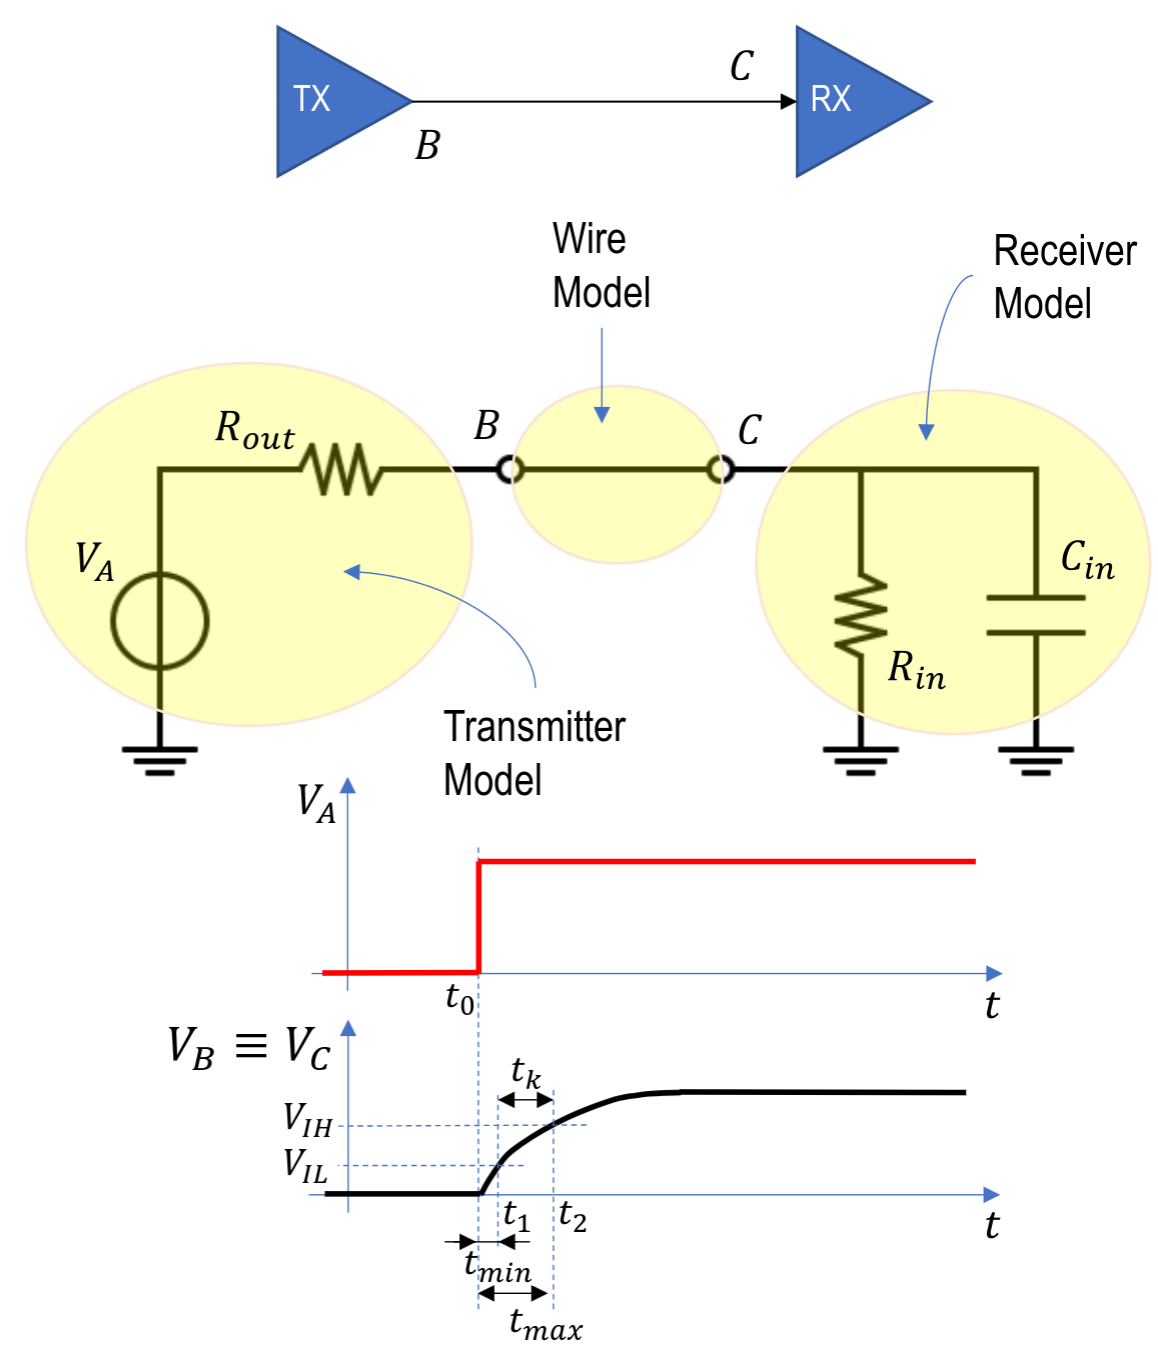
\includegraphics[scale=0.22]{../figures/skew.png}
\end{center}

The delay depends  on the receiving gate threshold, between $V_{IL}$ and $V_{IH}$.

We see that at the receiver we get an exponential ramp with time constant:
$$
\tau = C_{in} \cdot (R_{in} \parallel R_{out})
$$

Now, based on the input gate threshold, the delay time sits between $t_\text{min}$ and $t_\text{max}$:
$$
\begin{aligned}
	t_\text{min} &= t_1 - t_0 \\
	t_\text{max} &= t_2 - t_0 \\
\end{aligned}
$$
Where $t_1$ is where we meet $V_{IL}$ and $t_2$ is where we meet $V_{HL}$.

The \textbf{skew} $t_k$ is exactly:
$$
t_k = t_\text{max} - t_\text{min} = t_2 - t_1
$$

So we know that to correctly characterize the entire interconnection we have to:
\begin{itemize}
	\item Find the minimum of all minimum delays $t_\text{min}$;
	\item Find the maximum of all maximum delays $t_\text{max}$;
\item Compute the average $t_\text{avg}$ and skew $t_k$.
\end{itemize}
$$
\begin{aligned}
	t_\text{avg} &= \frac{t_\text{min} + t_\text{max}}{2} = \frac{t_1 + t_2 - 2 t_0}{2} \\
	t_k &= t_\text{max} - t_\text{min} = t_2 - t_1
\end{aligned}
$$

To summarize, we model an interconnection as lumped parasitic resistance $R_w$ and capacitance $C_w$.
The transmission shows a delay due to the input parasitic capacitance of the receiver, and due to the lumped parasitic capacitance of the wire.

The delay shows an \textit{uncertainty} (skew) due to different thresholds among nominally identical logic gates, and due to possibly different positions of the receiver along the interconnection wire.
In short, wire length causes different parasitic resistance $R_w$ and capacitance $C_w$ values, which affects both the delay and its uncertainty (skew).

\subsubsection{Models}

Let's see some popular models for delays in interconnects:
\begin{itemize}
	\item \textbf{\textsf{Exponential}} \\
Let's complete the previous model by putting the \textit{wire} back into the picture. As always, we model it with a parasitic capacitance and resistance:
\begin{center}
	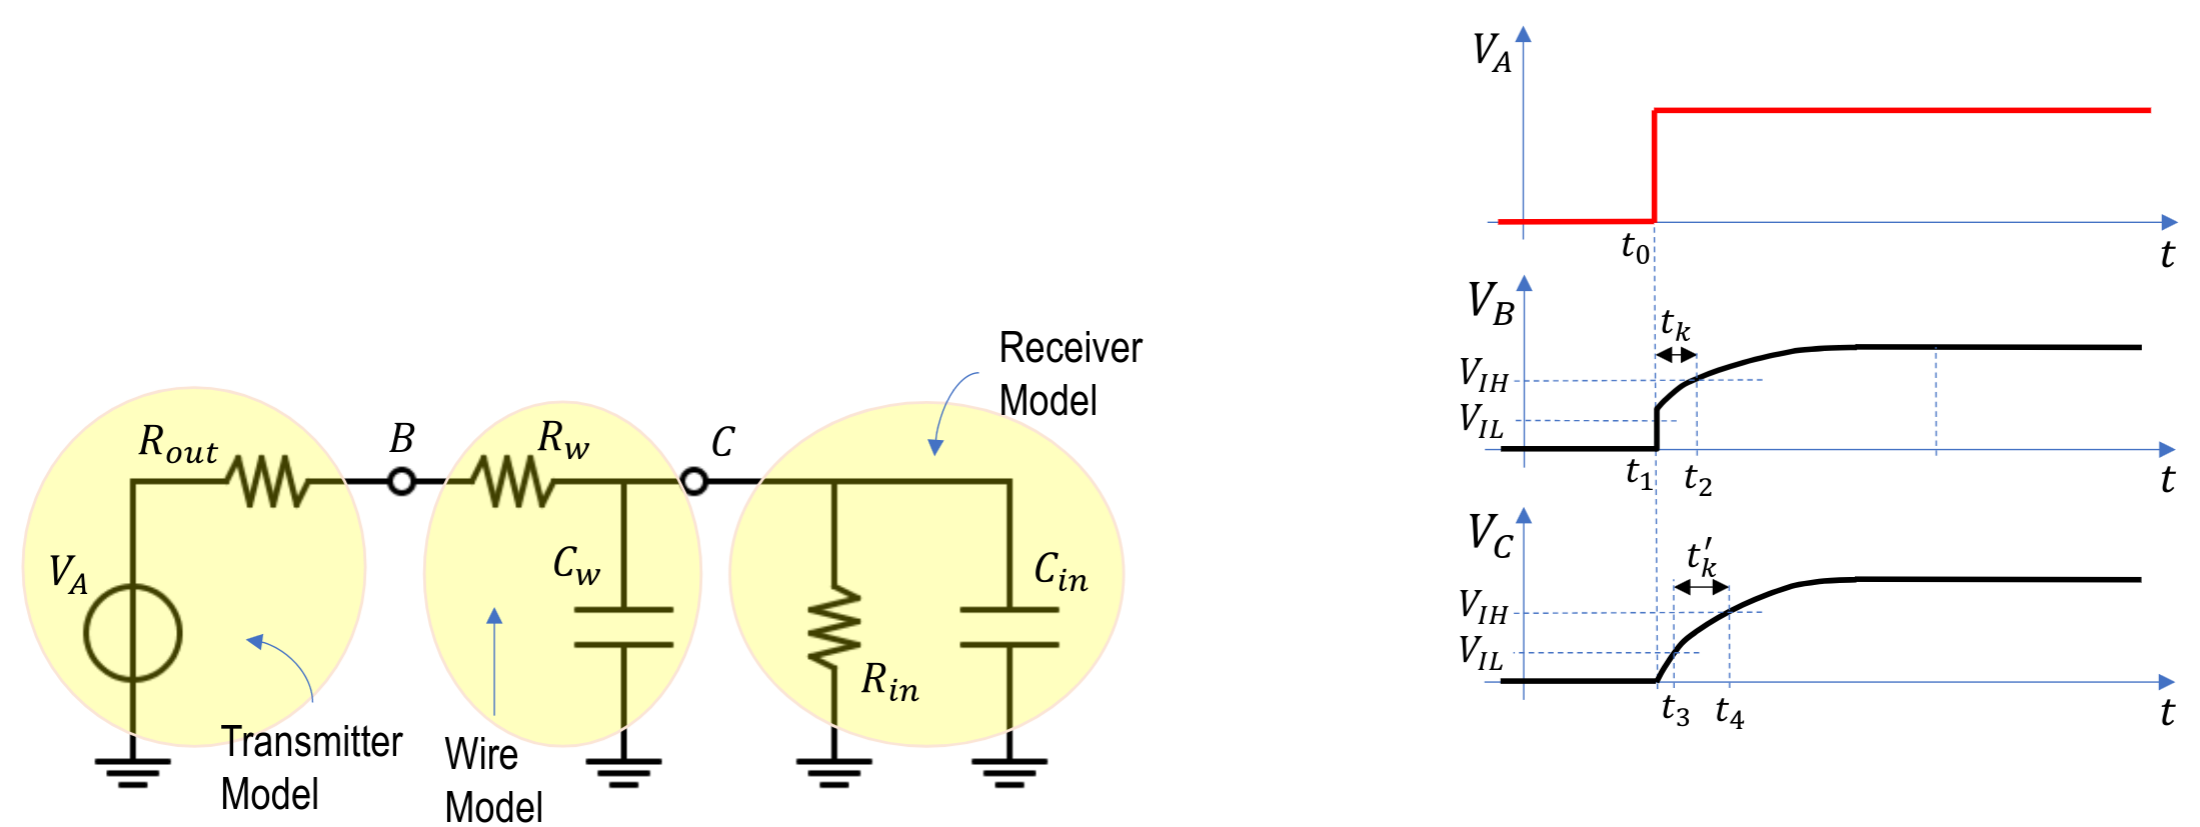
\includegraphics[scale=0.2]{../figures/skewire.png}
\end{center}

In this case our time constant changes:
$$
\tau = (C_\text{in} + C_w) \cdot (R_\text{in} \parallel (R_\text{out} + R_w) )
$$

Note that this situation is made even more complex by the fact that the wire constants $C_w$ and $R_w$ \textit{change} with the length of the wire, meaning that we have an added layer of uncertainty.

	\item \textbf{\textsf{Transmission lines}} \\
The idea is to model an interconnection using distributed parasitics: we take a wire and divide its length $l$ into $N$ segments, each lumped.
This means each segment has length $\Delta x = \frac{l}{N}$.
We are interested in what happens if we take the limit of elements going to infinity ($N \rightarrow + \infty$).

\begin{center}
	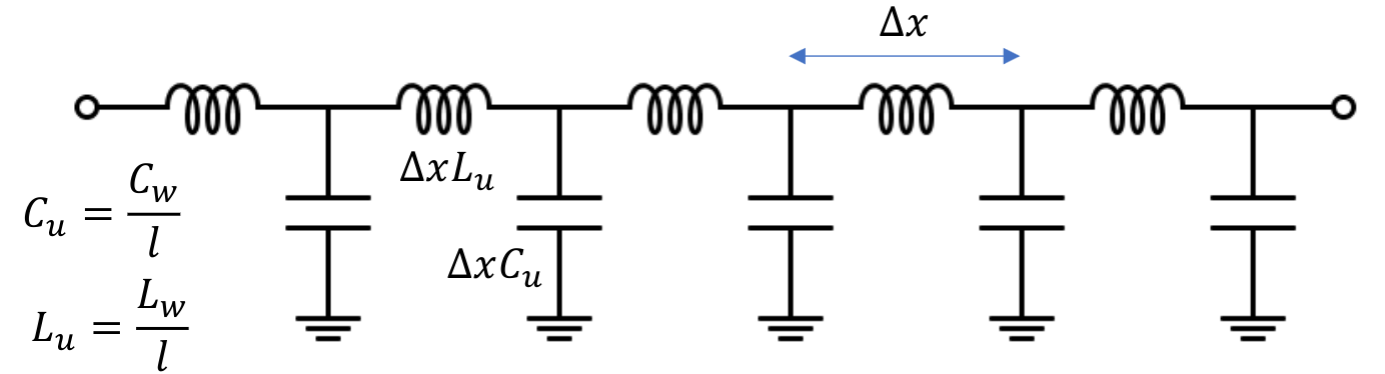
\includegraphics[scale=0.22]{../figures/trans_line.png}
\end{center}

If considering only inductance and capacitance, this is the \textbf{ideal transmission line with no losses}.
Signal propagates with a certain speed, with possible reflections, and the delay depends on the position of the receiver along the line.
For this we can compute an average and a skew.

Note that, if the resistances are also included, losses are introduced in the model and we get the \textbf{ideal transmission line with losses}.
	\item \textbf{\textsf{Elmore delay}} \\
Note that this already appeared in 7.0.2, for NAND topology memory timings.
There's a useful note here: \url{https://raw.githubusercontent.com/seggiani-luca/ees-notes/fcbb33c4bfdef8fc531aa81c04cddb69d309ad2a/notes/nand_topology_delay/main.pdf}.

The idea once again is to model an interconnection using distributed parasitics, by dividing the wire into $N$ segments, each with a lumped model.
For complex interconnections, we can determine a tree stemming from a single node $s$, where each segment is characterized by resistance $R_j$, and capacitance $C_j$.

\begin{center}
	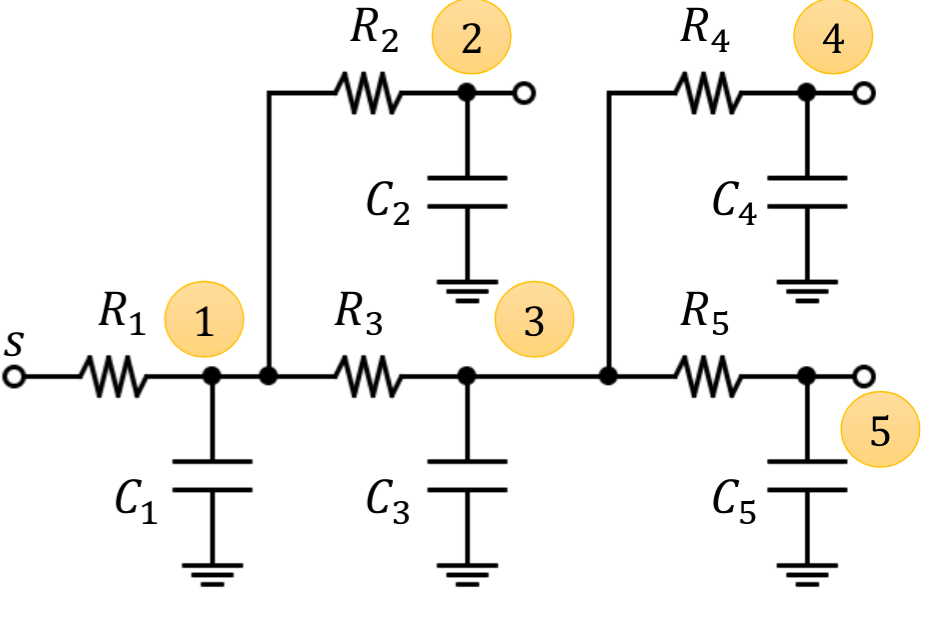
\includegraphics[scale=0.22]{../figures/elmore.png}
\end{center}
Matematically, the time constant $\tau_i$ of the delay at node $i$ is given by the sum of all RC segments up to $i$:
$$
\tau_i = \sum_{k = 1}^N C_j R_{ik}
$$
Where $R_{ik}$ is the shared path resistance between node $i$ and $k$:
$$
R_{ik} = \sum R_j \ \text{where} \ \left( R_j \in \text{path}(s, i) \cap \text{path}(s, k) \right)
$$

\item \textbf{\textsf{Elmore delay line}} \\

Elmore delay is easily applied to an RC segment line:

\begin{center}
	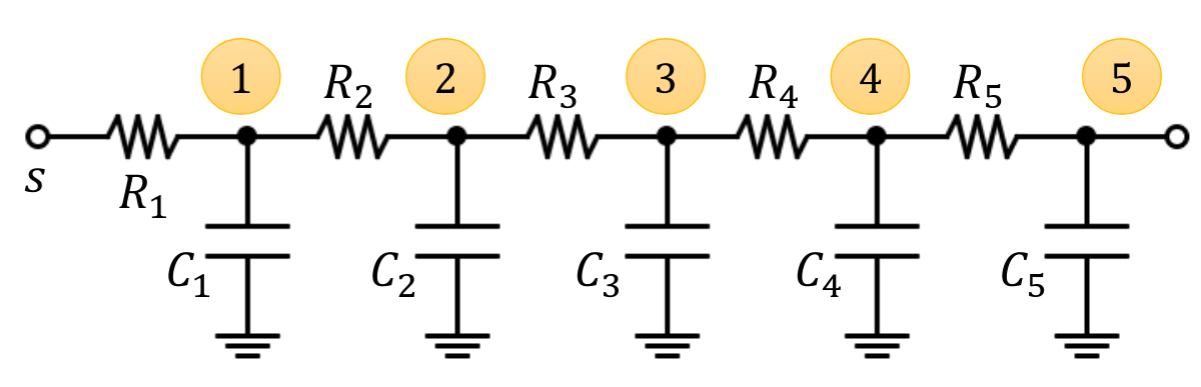
\includegraphics[scale=0.22]{../figures/elm_line.png}
\end{center}

The shared path resistance is always the sum of
all resistance between root $s$ and the considered node.
For the last node $i$ the shared path resistance with node $k$ is always:
$$
R_{ik} = R_{kk} = \sum_{j=0}^k R_j
$$

At this point we have that, for a wire of length $l$ divided into $N$ identical segments:
\begin{itemize}
\item All resistances are identical: $R_i = r \frac{l}{N}$ (where $r$ is the resistance per unit of length);
\item All capacitances are identical: $C_i = c \frac{l}{N}$ (where $c$ is the capacitance per unit of length).
\end{itemize}

This means we can apply Gauss's formula:
$$
\tau_\text{tot} = \tau_N = R_i C_i \frac{N(N + 1)}{2} = R_\text{tot} C_\text{tot} \frac{N + 1}{2N}
$$

In the limit this is:
$$
\tau \rightarrow \frac{1}{2} N^2 R_i C_i
$$

Where:
$$
\begin{aligned}
	R_\text{tot} = N R_i \\
	C_\text{tot} = N C_i
\end{aligned}
$$

Which should be the case we saw in our notes.

There is as slight notation difference between this in the notes:
\begin{itemize}
	\item In the notes we took each capacitor at contributing $t_i$ to the total delay time, thus giving:
$$
t_\text{tot} = \sum_i t_i
$$
\item Here we took $t_i$ as the delay at node $i$, already containing the delay from previous nodes (see the formula above for $\tau_i$), thus giving:
$$
t_\text{tot} = t_N
$$
\end{itemize}

Nevertheless, the result we get in both cases is the same, we just changed the definitions of the derivations.

\end{itemize}

\subsubsection{Parallel vs serial}

To transmit a word of $n$ bits, bits are transmitted according to a synchronization signal.
The synchronization signal is a clock, where:
\begin{itemize}
	\item The clock frequency is $f_\text{ck}$;
	\item The clock period is $t_\text{ck} = \frac{1}{f_\text{ck}}$. 
\end{itemize}
Note that the clock shall be transmitted as well as the signal.
There are several ways of communicating the clock.
We wish to compare these techniques based on throughput:
\begin{itemize}
	\item The number of bits per second is $\text{Thr}_\text{bits}$;
	\item The number of bits per second is $\text{Thr}_\text{words}$.
\end{itemize}

Assume the transmitted symbols represent single bits: we can increase performance by using multiple bits per symbol, thus lowering noise margins.

\begin{itemize}
	\item \textbf{\textsf{Parallel}} \\
This is the idea of \textbf{parallel}, as opposed to \textbf{serial}, transmission.
We transmit an entire word using $n$ parallel wires, with an additional wire for the clock.

This increases performance linearly:
\begin{itemize}
	\item The number of bits per second becomes $\text{Thr}_\text{bits} = n f_\text{ck}$;
	\item The number of bits per seconds stays $\text{Thr}_\text{word} = f_\text{ck}$, assuming the $n$ parallel lines form a complete word. Because of this, the number of bits is often a power of 2.
\end{itemize}

Parallel is certainly performant, but this comes at a cost we need a lot of wires for large busses, and its not good for long interconnections as its heavy, bulky, and of large size;
	
\item \textbf{\textsf{Serial}} \\
\textbf{Serial} is parallel's chill cousin, where we usually transmit the word and the clock using a single wire.
Bits are multiplexed in time, one per clock cycle, and one after the other, sequentially (LSB or MSB first).
This inevitably introduces latency at the word level.
A problem is also that the clock must usually be embedded in some way with the data, which needs special encodings for clock recovery.

The effects on performance are:
\begin{itemize}
	\item The number of bits per second becomes $\text{Thr}_\text{bits} = f_\text{ck}$;
	\item The number of bits per seconds becomes $\text{Thr}_\text{word} = \frac{ f_\text{ck}}{n}$, assuming again that $n$ is the number of bits in a complete word.
\end{itemize}

With them being mostly opposite, serial is way cheaper and simpler than parallel, if not a bit less performant.

\end{itemize}

\subsubsection{Clock}

There are limitations on the clock frequency.
The receiving end usually has flip-flops to store the incoming data: setup and hold times $t_s$ and $t_h$ must be satisfied at the receiving end.

Let's consider first a simplified model (no skew $t_k$), and then a more accurate one.

\begin{itemize}
	\item \textbf{\textsf{No skew}} \\
With no transmission delays and perfect synchronization,
the maximum $f_\text{ck}$ depends on $t_s$ and $t_h$ of the receiving flip-flops only:
$$
t_\text{ck} > t_s + t_h, \quad f_\text{ck} < \frac{1}{t_s + t_h}
$$

This is fine as, if clock and data have different (but known) delays, the transmitter properly produces the clock earlier or later so
that setup and hold times are satisfied at the receiver.


To satisfy these contraints we define 4 parameters:
\begin{itemize}
	\item $t_1^{TX}$: time the data is stable at the TX side before the active clock edge;
	\item $t_1^{RX}$: time the data is stable at the RX side before the active clock edge;
	\item $t_2^{TX}$: time the data is stable at the TX side after the active clock edge;
	\item $t_2^{RX}$: time the data is stable at the RX side after the active clock edge.
\end{itemize}

It must be that:
$$
t_1^{RX} \geq t_s, \quad t_2^{RX} \geq t_h
$$
	
\item \textbf{\textsf{Skew}} \\
Let's reintroduce skew. This means the delay is not the constant $t_\text{prop}$ (unknown but not significant) anymore, but a varying:
$$
t_d = t_\text{prop} \pm \frac{t_k}{2}
$$
Where $t_k$ is our skew.

With the phase delay between data and clock not maintained, delays are unpredictable and different in clock and data.
Delays change from one bit transmission to the next, and the transmitter should consider the worst case scenario.

For the setup time we have two sources of badness:
\begin{itemize}
\item Clock arrives early at RX after:
$$
t_d^{ck} = t_\text{prop} - \frac{t_k}{2}
$$
\item Data arrives late at RX after:
$$
t_d^{data} = t_\text{prop} + \frac{t_k}{2}
$$
\end{itemize}

$$t_1^{RX} = t_1^{TX} + t_d^{ck} - t_d^{data} = t_1^{TX} - t_k$$
Since it should be that $t_1^{RX} > t_s$, it has to be that:
$$
t_1^{TX} > t_s + t_k
$$

Via similar hold time considerations ($t_2$) we get the frequency constraint:
$$
f_\text{ck} < \frac{1}{t_s + t_h + 2 t_k}
$$

\end{itemize}

\end{document}
